\documentclass[11pt,a4paper,twocolumn]{article}

\newcommand{\EssayTitle}{No Place To Land}
%%%%%%%%%%%%%%%%%%%%%%%%%%%%%%%%%%%%%%%%%
% Wenneker Article
% Structure Specification File
% Version 1.0 (28/2/17)
%
% This file originates from:
% http://www.LaTeXTemplates.com
%
% Authors:
% Frits Wenneker
% Vel (vel@LaTeXTemplates.com)
%
% License:
% CC BY-NC-SA 3.0 (http://creativecommons.org/licenses/by-nc-sa/3.0/)
%
%%%%%%%%%%%%%%%%%%%%%%%%%%%%%%%%%%%%%%%%%

%----------------------------------------------------------------------------------------
%	PACKAGES AND OTHER DOCUMENT CONFIGURATIONS
%----------------------------------------------------------------------------------------

\usepackage[english]{babel} % English language hyphenation

%\usepackage{tgheros}
%\usepackage[black]{sourcesanspro}
% Use Montserrat only when explicitly requested (headings, etc.); keep serif body (XCharter) so italics work.
\usepackage[tabular,black]{montserrat}

\usepackage{microtype} % Better typography

%\usepackage{amsmath,amsfonts,amsthm} % Math packages for equations
\usepackage{amsmath,amsfonts} % Math packages for equations

\usepackage[svgnames]{xcolor} % Enabling colors by their 'svgnames'

% Define a color using HTML (hex) values
% https://en.wikipedia.org/wiki/Flag_of_Sweden
% Pantone 301C and Pantone 116C
\definecolor{yellow}{HTML}{FFCD00}
\definecolor{blue}{HTML}{004B87}

\usepackage[hang, small, labelfont=bf, up, textfont=it]{caption} % Custom captions under/above tables and figures

\usepackage{booktabs} % Horizontal rules in tables
\usepackage{tabularx} % Tables that automatically adjust column widths
\usepackage{listings} % Code listings
\lstset{
  basicstyle=\small\ttfamily,
  columns=fullflexible,
  keepspaces=true,
  frame=none,
  showstringspaces=false,
  tabsize=2
}

\usepackage{lastpage} % Used to determine the number of pages in the document (for "Page X of Total")

\usepackage{graphicx} % Required for adding images

\usepackage{enumitem} % Required for customising lists
\setlist{noitemsep} % Remove spacing between bullet/numbered list elements

\usepackage{sectsty} % Enables custom section titles
\allsectionsfont{\raggedright\usefont{OT1}{phv}{b}{n}} % Change the font of all section commands (Helvetica)




%----------------------------------------------------------------------------------------
%	MARGINS AND SPACING
%----------------------------------------------------------------------------------------

\usepackage{geometry} % Required for adjusting page dimensions

\geometry{
	top=1cm, % Top margin
	bottom=1.5cm, % Bottom margin
	left=2cm, % Left margin
	right=2cm, % Right margin
	includehead, % Include space for a header
	includefoot, % Include space for a footer
	%showframe, % Uncomment to show how the type block is set on the page
}

\setlength{\columnsep}{7mm} % Column separation width

%----------------------------------------------------------------------------------------
%	FONTS
%----------------------------------------------------------------------------------------

\usepackage[T1]{fontenc} % Output font encoding for international characters
\usepackage[utf8]{inputenc} % Required for inputting international characters

\usepackage{XCharter} % Use the XCharter font

%----------------------------------------------------------------------------------------
%	HEADERS AND FOOTERS
%----------------------------------------------------------------------------------------

\usepackage{fancyhdr} % Needed to define custom headers/footers
\pagestyle{fancy} % Enables the custom headers/footers
\setlength{\headheight}{26pt} % Avoid fancyhdr headheight warnings

\renewcommand{\headrulewidth}{0.0pt} % No header rule
\renewcommand{\footrulewidth}{0.4pt} % Thin footer rule

\renewcommand{\sectionmark}[1]{\markboth{#1}{}} % Removes the section number from the header when \leftmark is used

%\nouppercase\leftmark % Add this to one of the lines below if you want a section title in the header/footer

% Headers
\lhead{} % Left header
\chead{\textit{\EssayTitle}} % Center header - currently printing the article title
\rhead{} % Right header

% Footers
\lfoot{} % Left footer
\cfoot{} % Center footer
\rfoot{\footnotesize Page \thepage\ of \getpagerefnumber{LastPage}} % Right footer, "Page 1 of 2"

\fancypagestyle{firstpage}{ % Page style for the first page with the title
	\fancyhf{}
	\renewcommand{\footrulewidth}{0pt} % Suppress footer rule
}


% Same author-year bibliography and natbib-compatible citation commands as 10x.
\usepackage[backend=bibtex,style=authoryear,natbib=true,maxbibnames=99,useprefix=true]{biblatex}
\addbibresource{references.bib}
\AtBeginBibliography{\interlinepenalty=10000} % Keep each reference together.
\usepackage[autostyle=true]{csquotes}

\usepackage{tikz}
\usepackage{eso-pic}
\usetikzlibrary{fadings}
\usepackage{needspace}
\usepackage{etoolbox}
\usepackage[titles]{tocloft}
\usepackage{hyperref}
\hypersetup{
  colorlinks=true, linkcolor=blue, urlcolor=blue, citecolor=black,
  pdftitle={No Place To Land}, pdfauthor={Michel Blomgren},
  pdfsubject={AI-enabled capability, organizational recomposition, and co-invention},
  pdfkeywords={AI, customer value, organizational productivity, co-invention, C89 Systems},
  bookmarksopen=true, bookmarksnumbered=false, bookmarksdepth=2
}

\definecolor{CoverBlue}{HTML}{8ACFFF}
\definecolor{CoverInk}{HTML}{020713}
\newcommand{\CoverImage}{cover.png}
\newcommand{\CoverTopShade}{0.12}
\newcommand{\CoverBottomShade}{0.72}
\newcommand{\CoverFadeTop}{0.36\paperheight}
\newcommand{\CoverFadeBottom}{0.24\paperheight}
\tikzfading[name=coverFade,bottom color=transparent!0,top color=transparent!100]

\setcounter{secnumdepth}{0} % Manuscript chapter numbers are part of their headings.
\setcounter{tocdepth}{1}    % Keep the contents at chapter level.
\renewcommand{\cftsecleader}{\cftdotfill{\cftdotsep}}
\setlength{\cftbeforesecskip}{9pt}
\pretocmd{\section}{\Needspace{7\baselineskip}}{}{}
\pretocmd{\subsection}{\Needspace{5\baselineskip}}{}{}
\lfoot{\footnotesize\href{https://c89.systems}{C89 Systems}}

\begin{document}
\onecolumn
\thispagestyle{firstpage}

% Full-bleed artwork and a tunable bottom fade protect the abstract's contrast.
\AddToShipoutPictureBG*{%
  \AtPageLowerLeft{\includegraphics[width=\paperwidth,height=\paperheight]{\CoverImage}}%
  \begin{tikzpicture}[remember picture,overlay]
    \fill[CoverInk,opacity=\CoverTopShade]
      (current page.south west) rectangle (current page.north east);
    \fill[CoverInk,opacity=\CoverBottomShade,path fading=coverFade]
      ([yshift=\CoverFadeBottom]current page.south west)
      rectangle ([yshift=\CoverFadeTop]current page.south east);
    \fill[CoverInk,opacity=\CoverBottomShade]
      (current page.south west)
      rectangle ([yshift=\CoverFadeBottom+0.1pt]current page.south east);
  \end{tikzpicture}%
}

% All cover copy and branding remain native typeset text and vector artwork.
\begin{tikzpicture}[remember picture,overlay]
  \node[anchor=north west,inner sep=0pt]
    at ([xshift=20mm,yshift=-17mm]current page.north west)
    {\includegraphics[width=43mm]{assets/c89-systems.pdf}};
  \node[anchor=north west,inner sep=0pt,text width=170mm]
    at ([xshift=20mm,yshift=-43mm]current page.north west) {%
      \raggedright\color{CoverBlue}
      {\fontsize{56}{59}\usefont{T1}{Montserrat-TLF}{b}{n}No\hspace{0.25em}Place\\To\hspace{0.25em}Land\par}
      \vspace{7mm}
      {\large\usefont{OT1}{phv}{b}{n}\color{white}Michel Blomgren\par}
      \vspace{1.5mm}
      {\small\usefont{OT1}{phv}{m}{n}\color{CoverBlue}
        \hypersetup{urlcolor=CoverBlue}\href{mailto:mike@c89.systems}{mike@c89.systems}\par}
    };
  \node[anchor=south west,inner sep=0pt,text width=170mm]
    at ([xshift=20mm,yshift=18mm]current page.south west) {%
      \color{white}
      {\small\usefont{OT1}{phv}{b}{n}\color{CoverBlue}ABSTRACT\par}
      \vspace{3mm}
      {\fontsize{11}{14}\selectfont\noindentThis essay examines why expanding AI-enabled capability does not
automatically become customer value or organizational productivity.
Drawing on innovation economics, organizational theory, and contemporary
AI research, it extends \emph{The Coordination Shift} from changes in
the production unit to the conditions required to employ it. It argues
that capability can outpace both the conception of worthwhile uses and
the authority, investment, and commercial relationships needed to
sustain them. Organizational recomposition and reusable co-invention
offer a practical response: developing not only the means of production,
but the organizational and commercial capacity to put them to use.
\par}
    };
\end{tikzpicture}
\null
\clearpage

\tableofcontents
\vfill
\begin{center}
  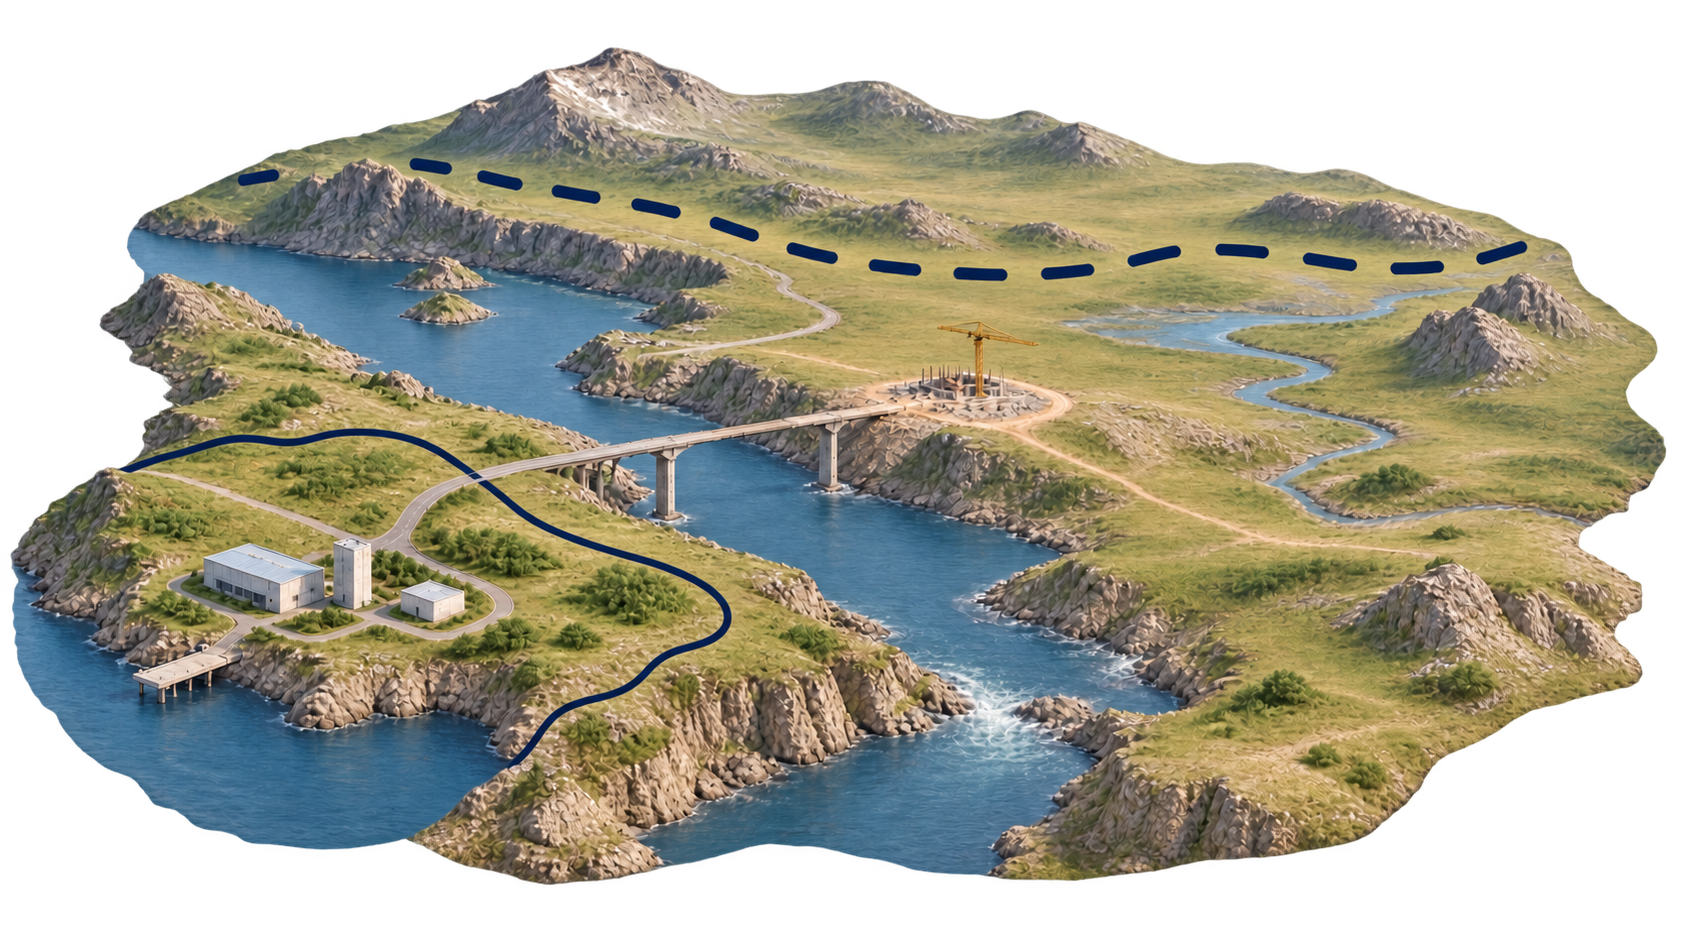
\includegraphics[width=165mm]{frontier-landscape-v2.png}\par
  \vspace{2mm}
  {\small
    \tikz[baseline=-0.5ex]{\draw[blue,line width=1.2pt] (0,0)--(10mm,0);}%
    \enspace Sustained use\qquad
    \tikz[baseline=-0.5ex]{\draw[blue,line width=1.8pt,dash pattern=on 3pt off 3pt] (0,0)--(10mm,0);}%
    \enspace Capability frontier\par
  }
\end{center}
\vfill
\noindent\includegraphics[width=24mm]{assets/c89-systems-black.pdf}%
\hfill{\footnotesize\textbf{Michel Blomgren}\quad\href{mailto:mike@c89.systems}{mike@c89.systems}}\par
\vspace{2mm}
\noindent{\footnotesize This essay extends \textit{The Coordination Shift}, available as
\href{https://c89.systems/10x.pdf}{PDF} and
\href{https://c89.systems/10x.md}{Markdown}.}\par

\twocolumn
\section{Introduction}\label{introduction}

A business can recognize a valuable improvement and still have no
workable way to commission it. The people who need the result may not
control the systems, decisions, or budgets required to produce it. An
engineer who can connect those pieces technically cannot necessarily
connect them organizationally. A better solution can therefore leave the
business no closer to using it, and a more capable engineer no closer to
obtaining a suitable assignment.

\emph{The Coordination Shift} \citep{blomgren2025coordination} argued
that AI changes the effective unit of work. In suitable domains, an
experienced person working with agents can coordinate design,
implementation, verification, and operation across a scope that
previously required a larger human team. That changes the feasible
division of labour, not just the speed of individual tasks. \emph{No
Place to Land} follows the resulting producer into the organizations and
markets through which its work is assigned, authorized, financed, and
purchased.

The subject is a capability to combine and operate technologies, rather
than a particular invention seeking a market. Its owner experiences
productive leverage: more can be accomplished with the resources
available. The customer evaluates a different proposition: what becomes
possible or better as a consequence. Lower expenditure, less
coordination, a more dependable service, or an activity previously too
expensive to pursue can each provide a reason to buy. The use itself may
have to be conceived and demonstrated before the customer can formulate
it as a requirement.

The bet of this essay is that the expansion of small-unit capability
will make the connections between production, customer value, and
institutional capacity increasingly decisive. A unit may be able to
deliver an integrated result while its prospective employer or customer
can commission only separate contributions. Making the benefit
understandable does not automatically make it obtainable. Conversely,
greater freedom to operate cannot rescue an offering that provides
insufficient benefit. These are interacting problems, with different
remedies.

Widespread AI use is compatible with that mismatch. Internetstiftelsen's
\emph{Svenskarna och internet 2026}
\citep{internetstiftelsen2026internet} describes substantial workplace
adoption alongside uneven perceived efficiency gains. The research
examined here also includes positive operating results and experiments
that change the combination of people and machines producing an output.
Those observations do not settle the organization of future production.
A company can improve work inside its existing roles while leaving the
responsibilities surrounding those roles largely unchanged.

\emph{Organizational recomposition} means reconsidering that grouping of
work, including the authority and accountability attached to it. It asks
which activities and handoffs remain necessary once a different unit can
carry the result. The historical literature on co-invention
\citep{bresnahan1996coinvention} provides a foundation: the surrounding
production system is part of what must be invented. AI changes the
urgency of that work when executable scope expands faster than the
assignments and commercial relationships available to employ it.

The argument is a prospective synthesis, grounded in established
mechanisms and contemporary evidence. It does not require every firm to
become small or every existing role to disappear. A compact human--AI
unit can operate inside a large enterprise, and an incumbent may supply
precisely the demand and resources an independent producer lacks. AI can
also help construct the integration and operating knowledge that make
adoption easier. The capability to produce and the capacity to put
production to use can both improve, without improving at the same rate.

The practical question is how engineers, entrepreneurs, and
organizational leaders act while that adjustment is incomplete. The
chapters that follow examine why useful capability remains difficult to
employ, how unfamiliar possibilities become customer value, and what
makes those benefits purchasable and sustainable. The destination is a
strategy for constructing a workable route into production, rather than
waiting for the surrounding economy to request the future in the form of
a specification.

\section{1. The Persistent Gap Between Capability and
Value}\label{the-persistent-gap-between-capability-and-value}

After the dot-com crash, while applying for jobs, I met a founder who
gave me an unusually candid answer. As I remember it, he would have
liked to employ people with deep technical ability, but there was no
business for that capability at the time. The distinction stayed with
me: appreciating what someone can do does not create an economic setting
in which they can do it. Technical capacity and a viable place to employ
it are separate achievements.

This need not reflect a failure of understanding on either side. A
business needs work it can commission, a way to incorporate the result,
and sufficient benefit to sustain the commitment. An engineer may
understand an operational problem and know how to solve it without
having access to that combination. The founder's response was an
instance of a wider question: what separates an available capability
from its productive employment?

\subsection{The system around the
invention}\label{the-system-around-the-invention}

In \emph{The Dynamo and the Computer} \citep{david1990dynamo}, Paul
David examined why electrification and computing did not immediately
yield the productivity gains their possibilities suggested. Early
factory retrofits often retained shaft-and-belt transmission. Individual
electric motors subsequently permitted different layouts, materials
handling, and maintenance arrangements. Capturing those advantages
depended on investment, replacement economics, and application
experience, not simply access to a different power source. Engineers
could anticipate improvements before the conditions for implementing
them widely existed.

David also identified a reason information structures might be less
readily renewed than physical machinery. What a firm records, how
information circulates, and how it is interpreted need not become
progressively more expensive to maintain simply because it is old.
Physical wear does not force the replacement of an information system in
the same way. The analogy therefore offers no assurance that time alone
will produce transformation; it directs attention to the circumstances
and work through which a different productive system emerges.

Erik Brynjolfsson and Lorin Hitt's \emph{Beyond Computation}
\citep{brynjolfsson2000computation} brought together case studies and
firm-level analyses linking returns from information technology to
organizational investment. Evidence of firm-level benefits preceded the
aggregate productivity acceleration then becoming visible. Benefits
could be real, unevenly distributed, and difficult to identify in
economy-wide statistics at the same time. The presence of computers was
a poor description of the productive system an organization had
developed around them.

These accounts establish that invention, effective use, and measured
results need not move together. They do not supply a timetable for AI.
Their more durable lesson is that the receiving organization belongs
inside the explanation of technological performance: replacing a working
technology with a better version does not necessarily complete the
organizational work required to exploit it.

\subsection{Different gaps, different
consequences}\label{different-gaps-different-consequences}

Technical capability concerns what can be accomplished under specified
conditions. Productivity concerns output relative to the resources
required to produce it. Customer value concerns what the recipient
gains, taking account of what they must give up. Commercial returns
concern what particular participants retain after their costs. A
reduction in engineering effort can affect all four, but it need not
affect them equally or simultaneously.

Consider an analyst who prepares an internal report more quickly. The
saving can be real even if the report enters the same monthly decision
cycle and no additional decisions are made. Reduced overtime, better
quality, or capacity released for other work may still be valuable. The
capacity may also remain unused. Measuring preparation time establishes
the local change; determining its wider consequence requires following
what happens beyond that activity. An impressive improvement in an
infrequent task can have less effect on total output than a smaller
improvement at a persistent constraint.

Brynjolfsson, Daniel Rock, and Chad Syverson distinguish four
explanations for the gap between technological expectations and measured
results in their analysis of the modern productivity paradox
\citep{brynjolfsson2019paradox}: mistaken expectations, measurement
problems, redistribution, and implementation delays. They emphasize the
time required for complementary innovations and organizational
adjustments while allowing several explanations to operate together. An
account of AI productivity should preserve that distinction rather than
assign every disappointing result to slow adoption.

Their \emph{Productivity J-Curve} \citep{brynjolfsson2021jcurve}
explains how investment in intangible complements changes the timing of
measured productivity. Resources devoted to developing future capability
may be counted without adequately recording the asset being created.
Productivity growth can then be understated during investment and
overstated when the benefits of previously unmeasured assets are
harvested. Building the means to use a technology can look unproductive
before that work pays off.

That is different from possessing a capability for which nobody is
making the complementary investment. One organization is constructing a
future production system; another has acquired tools without a
commitment to change how it operates. Both can show limited immediate
gains, but completing an investment and initiating one are different
problems. Calling both an implementation lag conceals the decision still
missing in the second case.

David Teece adds a separate question in \emph{Profiting from
Technological Innovation} \citep{teece1986innovation}. Customers,
imitators, or owners of complementary assets may benefit while the
innovator captures little of the return. Productive capability that
remains unused must therefore be distinguished from productive
capability whose benefits accrue elsewhere. A better route to customers
might address either problem, but a higher price alone cannot turn
unused capacity into useful production.

\subsection{When the producer moves
ahead}\label{when-the-producer-moves-ahead}

The changed unit described in \emph{The Coordination Shift} brings this
historical problem closer to the individual practitioner. Suppose an
engineer can coordinate a complete integration, including its
verification and operation, but is employed only to implement one
component. The broader capability is available; the broader assignment
is not. Starting a company changes who directs the work internally
without automatically supplying customers, operating access, or
authority over the dependencies outside it.

The delay is then not simply between a laboratory invention and adoption
across an industry. It occurs between a feasible producer and the work
that producer can obtain. The problem may already be understood, and the
mechanism may already work. What remains unavailable is the combination
of decisions and commitments through which its use becomes economically
sustainable.

A widening gap is also compatible with rising productivity. If
businesses adopt new capabilities while feasible applications expand
faster, they can produce more and leave more unrealized. This is a
conditional relationship, not a measured inventory of forgone output. It
explains why successful adoption does not by itself establish that the
distance between productive possibility and practical use is closing.

AI sharpens the question raised by the founder's response. When
execution capacity can increase within a small unit without a
corresponding change in the surrounding business, more engineering
ability need not resolve the next constraint. The work required between
a feasible mechanism and dependable production becomes part of the
innovation itself.

\section{2. Co-Invention: Why Technology Is Never the Whole
System}\label{co-invention-why-technology-is-never-the-whole-system}

Consider a hypothetical reconciliation service that matches records
across two business systems, identifies discrepancies, and applies
corrections under specified rules. Assume its technical behaviour has
been demonstrated for a defined class of transactions, including
interruption and recovery. The business nevertheless retains its manual
procedure because the departments concerned have not agreed when the
service's evidence can close a case or replace an existing check. The
technical result is available, but the organization has not established
how to rely on it.

The remaining work includes deciding how disputed records are resolved,
which corrections are permitted, and what happens outside those limits.
Some existing checks may remain necessary; others may duplicate evidence
the service already provides. These decisions establish the operating
method. They cannot be completed solely by improving matching accuracy
or documenting the old process more thoroughly.

\subsection{Invention at the point of
use}\label{invention-at-the-point-of-use}

Timothy Bresnahan and Shane Greenstein describe this complementary work
as \emph{co-invention} in their 1996 study of business computing
\citep{bresnahan1996coinvention}. Examining the transition from
mainframes to client/server systems, they include changes in
organizational purpose, jobs, hierarchies, and information flows within
the innovation process. Their findings challenge explanations centred on
vendor lock-in or obstructive information-systems departments.
Rebuilding deeply embedded applications was difficult inventive work
even where the new technology offered substantial benefits.

Co-invention is more than specifying requirements for an otherwise
complete solution. Describing how employees compare records, prepare
reports, and obtain approvals would not determine whether reconciliation
should retain that sequence. A new service might provide a different
basis for accepting corrections or resolve discrepancies before a
periodic report is needed. The intended use and the means of delivering
it must be developed together.

The division between technical and non-technical work is equally
inadequate. A decision about permitted corrections can be implemented as
an access control; an agreement about acceptable evidence can inform a
verification check; a continuity requirement can be embodied in a
recovery protocol. Each connects an operating judgment to executable
behaviour. Domain knowledge establishes what the system should mean and
permit, while engineering makes those decisions dependable in operation.
Neither side can complete the whole contribution by handing the other a
description of its own part.

A mechanism can consequently be complete for specified conditions while
its application remains unfinished. The missing work may concern
conditions that only the customer can authorize or facts that only its
operators possess. This does not negate the technical achievement. It
identifies what must still be supplied before the achievement becomes an
operating capability.

\subsection{Changes that work
together}\label{changes-that-work-together}

Paul Milgrom and John Roberts give this relationship an economic
formulation in \emph{Complementarities and Fit}
\citep{milgrom1995complementarities}. Choices are complementary when
increasing one raises the return to increasing another. Technology,
strategy, and organizational practices can therefore require joint
evaluation: the payoff to one change depends on the configuration in
which it is made.

Faster discrepancy detection is more useful when the business can
resolve the resulting cases promptly. Reliable transaction identifiers
improve automated matching; agreed evidence requirements increase the
usefulness of both. If detection accelerates while every case still
requires a scarce employee to reconstruct its history, the immediate
effect may be a longer queue. Improving one activity does not
necessarily improve the conditions governing completion.

The relevant comparison is therefore sometimes between combinations of
changes. Matching alone can appear unattractive, while matching combined
with evidence, bounded correction, and exception ownership has different
economics. In the latter design, an internal discrepancy report may
become unnecessary for ordinary cases. The opportunity extends beyond
performing each inherited task faster.

This does not make adoption an all-or-nothing exercise. Read-only
reconciliation may provide useful benefits without transferring
correction authority and may be a sensible way to establish confidence.
A staged approach is coherent when each stage has a worthwhile purpose
and the dependencies of the larger result are understood. It becomes
misleading when the benefits of the completed system are attributed to
an isolated component that cannot provide them.

\subsection{What a pilot establishes}\label{what-a-pilot-establishes}

A pilot can temporarily supply dependencies that have not been
established for ordinary operation. Carefully prepared data, immediate
answers from an experienced employee, and exceptional access approved by
a sponsor may be appropriate conditions for testing feasibility. They
nevertheless contribute to the result. A successful trial does not show
that their continued provision has become routine or affordable.

If a specialist privately resolves every ambiguous case, the trial has
not demonstrated independent resolution. If a sponsor personally obtains
every permission, it has not demonstrated repeatable authorization. If
recovery depends on the original developer's memory, it has not
established continuity beyond that person. Recording these contributions
separates technical performance from the cost of sustaining the service.

The trial remains useful when it reveals those requirements.
Co-invention turns what it teaches into an operating method: encoding
repeatable knowledge, retaining judgment where it is necessary, and
replacing temporary accommodations with dependable responsibilities. The
objective is not to eliminate every human contribution but to make the
contribution explicit and economically supportable.

\subsection{Knowledge that travels}\label{knowledge-that-travels}

Eric von Hippel's \emph{``Sticky Information'' and the Locus of Problem
Solving} \citep{vonhippel1994sticky} examines information that is costly
to acquire, transfer, and use elsewhere. Responses include moving
problem solving closer to the information, iterating between locations,
and changing how the problem is divided. Extracting a complete
specification for a remote designer is only one possible approach, and
can be the expensive one.

In the reconciliation example, a field labelled ``customer reference''
may have different meanings in the two systems. A discrepancy may
represent a legitimate timing difference rather than an error. An
experienced employee can recognize those distinctions without having
expressed them as exhaustive rules. The engineer, meanwhile, may see
ways of resolving them that the old procedure never allowed. Useful
design brings both kinds of knowledge to bear on actual cases.

Von Hippel also considers making repeatedly needed knowledge easier to
transfer. His custom-chip example describes encoding supplier
constraints in design tools so users can undertake more application
problem solving themselves. The location of problem solving
\citep{vonhippel1994sticky} can change without requiring every user's
information to become generic. A supplier can transfer a way to solve
local problems rather than first collecting every local problem
centrally.

For the systems considered here, common mechanisms can provide state
handling, authentication, recovery, and diagnostic evidence. Knowledge
of a recurring problem class can inform mappings, exception categories,
and acceptance checks. Local facts and commitments establish which
records are authoritative and who may decide disputed cases. A
deployment combines all three, but they do not transfer in the same way.
One customer's permission cannot travel with the software; a tested
method for defining and verifying a permission boundary can.

\subsection{Co-invention under AI}\label{co-invention-under-ai}

Bresnahan and Manuel Trajtenberg's theory of general-purpose
technologies \citep{bresnahan1995gpt} explains how improvements in a
widely used technology can make downstream innovation more productive
while leaving coordination problems between producers and users
unresolved. Better general capability expands the application
possibilities. Application remains inventive work.

The extension proposed here has two directions. When AI reduces the
effort needed to build and test a mechanism, unresolved application work
becomes a larger part of the remaining cost. Further execution capacity
provides little immediate benefit if the same unavailable operating
decision prevents deployment. Yet AI can also help compare inconsistent
records, explore designs, generate verification cases, and adapt
previously developed integrations. Investigation and implementation may
be coordinated within a smaller unit instead of passing through several
specialist groups.

This distinction prevents a static account of an accelerating technology
confronting permanently slow organizations. Both sides can improve. What
cannot be assumed is that improvements in analysis supply the
commitments analysis identifies. Software can expose contradictory
interpretations of a record; the parties responsible for the business
must still settle which interpretation governs their actions.
Co-invention joins those decisions to a dependable production method.
The contemporary evidence must therefore be read for what it observes
along that connection, not only for whether people have acquired a tool.

\section{3. AI Inside Yesterday's
Organization}\label{ai-inside-yesterdays-organization}

Contemporary AI studies examine different changes: providing an
assistant, integrating suggestions into an existing service, or altering
the combination of people and machines producing an output. Surveys add
observations about adoption, perceived benefits, and business results.
These findings become more useful when the operating arrangement is
identified before its performance is interpreted. They are not estimates
of a single treatment called organizational transformation.

Three dates also matter: when research was published, when its
observations were collected, and which technology and work practices
those observations concern. A study published during the current
transition may examine a much earlier configuration. Its result remains
evidence about that configuration, rather than a ceiling on every
subsequent way of producing.

\subsection{Adoption and operating
depth}\label{adoption-and-operating-depth}

Internetstiftelsen's \emph{Svenskarna och internet 2026}
\citep{internetstiftelsen2026internet} reports that 56\% of employed
respondents used AI for work in its January 2026 fieldwork, including
more than seven in ten white-collar workers. The use measure included
dedicated services and AI overviews in search, broadening the previous
year's definition. It establishes widespread use while grouping together
markedly different levels of engagement.

Among workplace AI users, six in ten said it helped them get more done.
Additional checking and rework were the most common explanations among
those reporting no efficiency improvement. Separately, 31\% of employed
respondents did not know whether their employer permitted dedicated AI
services. Perceived efficiency is not firm productivity, and permission
awareness is not a measure of organizational redesign. The survey shows
benefits, costs, and uncertainty within current work; it does not
identify the production boundaries behind them.

The UK Office for National Statistics distinguishes adoption from extent
of use in its 2026 business analysis \citep{ons2026businesses}. Among
AI-using businesses with at least ten employees, 10\% reported extensive
use in June 2026. ONS describes these newly introduced questions as
early indications. Nevertheless, they address something a count of
adopters misses: occasional availability and extensive operational use
are different conditions.

Microsoft's 2026 Work Trend Index \citep{microsoft2026wti} goes further
into organizational conditions. Its survey covered 20,000 AI-using
knowledge workers across ten markets. A readiness index, calculated for
the 16,971 respondents with complete data, classified 10\% as
experiencing ``blocked agency'': relatively high individual capability
alongside weaker organizational conditions. Both dimensions were
self-reported composites, not independent assessments of competence or
estimates of lost output.

These sources describe related but distinct properties. An employee can
receive encouragement to experiment without authority to change an
operating process. A firm can use AI extensively while retaining the
same decision rights. A narrowly deployed system can instead support a
substantial change in who owns one result. Incidence, intensity, and
authority should therefore be examined separately.

\subsection{Gains within the
assignment}\label{gains-within-the-assignment}

Eleanor Dillon and colleagues' \emph{Shifting Work Patterns with
Generative AI} \citep{dillon2025workpatterns} examines randomized
Microsoft 365 Copilot access among 7,137 workers across 66 firms. The
experiments ran during 2023--2024, with six months of assigned access
within firms. In the later months, assignment reduced weekly
email-application time by about 1.4 hours on average. The researchers
detected no change in the quantity or composition of measured
activities. Their telemetry observed application use rather than work
content or direct performance measures. Individual tool access, not a
reassigned production mandate, was the randomized intervention.

An operating study observes a different benefit. In \emph{Generative AI
at Work} \citep{brynjolfsson2025work}, Erik Brynjolfsson, Danielle Li,
and Lindsey Raymond study staggered deployment of a contextual assistant
among 5,172 customer-support agents. They estimate a 15\% average
increase in issues resolved per hour, with substantial variation across
workers. Here the result concerns completed service output, not
application time, within an established support operation.

The support case is consistent with an inherited organization already
supplying enough context, access, and acceptance for useful gains,
although those complements were not independently tested. Recomposition
is not a prerequisite for every improvement. The further question is
whether improving a component captures the available opportunity or
whether a different grouping of work becomes preferable as capability
broadens.

\subsection{A different production
unit}\label{a-different-production-unit}

The P\&G experiment in \emph{The Cybernetic Teammate}
\citep{dellacqua2026teammate} changes both tool access and human
composition. Conducted in 2024 and published in 2026, its analysis
covers 791 professionals working individually or in cross-functional
pairs, with or without AI, on real product-innovation challenges.
AI-assisted individuals performed comparably to unaided pairs on
proposal quality and produced more balanced technical and commercial
content. AI-assisted pairs were more likely to produce top-decile
proposals.

The output was an early-stage proposal from a one-day virtual workshop,
not a launched product or continuing operating responsibility. Within
that boundary, however, the experiment makes an organizational choice
available: which combination of human expertise is required for the
output? It is more than a test of whether one employee writes faster.

The prospective argument begins where that comparison ends. If a smaller
unit can reliably integrate formerly distributed knowledge, its feasible
responsibility can extend beyond the former individual assignment.
Whether that is useful depends on the result, constraints, and
continuing obligations. Holding the old division of labour fixed would
prevent examination of the organizational choice in the first place.

\subsection{Different economic
outcomes}\label{different-economic-outcomes}

Anders Humlum and Emilie Vestergaard's \emph{Still Waters, Rapid
Currents} \citep{humlum2026currents}, revised in March 2026, links
Danish adoption surveys to administrative records across eleven
occupations, with labour outcomes through December 2024. The researchers
report task reorganization alongside no detectable average effects on
earnings or recorded hours, with estimates precise enough to exclude
effects larger than 2\%. They also identify occupational movement among
adopters that is not yet large enough to shift average earnings.

The observed task changes include content generation, AI oversight, and
integration. These are changes in work, but not necessarily changes in
the accountable unit. Likewise, unchanged earnings do not establish
unchanged output. A firm can use released capacity without altering
compensation, while a worker can gain time without producing more market
output. Administrative labour measures do not resolve those
alternatives.

\emph{Firm Data on AI} \citep{yotzov2026firmdata} asks more directly
about business results. Based on surveys of nearly 6,000 executives in
four countries during late 2025 and early 2026, its March revision
reports that 89\% attributed no effect on sales volume per employee to
AI over the preceding three years. The denominator includes
non-adopters. This is executives' retrospective attribution, not an
independently identified causal effect on productivity, and it is
distinct from their expectations of future gains.

The OECD's late-2024 SME survey \citep{oecd2025smeworkforce} examines
another boundary. Among generative-AI users, 83\% reported no change in
overall staff needs, while 14.3\% reported reduced reliance on external
contractors and 6.3\% increased reliance. Those are reported directions,
not magnitudes of employment or expenditure. Unchanged internal staffing
needs can coexist with a change in what the business buys externally.

These observations concern different transmission paths. A unit can
produce more, bring work inside, release time, or require new
implementation assistance. How gains reach wages, revenue, or suppliers
depends on what happens along those paths. The evidence should be used
to locate the change, rather than compressed into a verdict that AI
either works or does not.

\subsection{When the measurement unit
changes}\label{when-the-measurement-unit-changes}

METR's February 2026 developer-productivity update
\citep{becker2026experiment} describes increasing difficulty retaining
participants willing to work without AI, changes in submitted tasks, and
problems attributing time when developers use agents concurrently. The
researchers judged their follow-up data an unreliable estimate of the
current productivity effect. Their account establishes measurement and
selection difficulties, not a dependable replacement speedup figure.

A fixed-task comparison and a production-system comparison answer
different questions. An operator may delegate one component while
investigating another, or undertake useful work previously too expensive
to justify. Timing an isolated issue misses part of that change.
Counting generated tests, documents, or features can exaggerate it if
the additional artifacts have little value. Neither measure alone
describes the effectiveness of the new system.

For the broader comparison proposed here, the customer objective and
required constraints should remain comparable while the deliverable and
production method are allowed to change. Evaluation should include
accepted outcomes, human attention, waiting, verification, and recovery
over a meaningful period. Where the claimed benefit is newly viable
work, the alternative can be not undertaking that work at all. This
aligns the measurement with the proposition being tested rather than
preserving yesterday's task inventory by definition.

\subsection{The setting around the
result}\label{the-setting-around-the-result}

The P\&G experiment supplied real business challenges and an evaluation
process developed with company leadership. That made a meaningful
production comparison possible. The essay asks an additional question:
how does a capable internal unit or independent supplier obtain the
work, information, authority, and acceptance that such a setting
provides?

Demonstrating performance inside a workable setting and constructing
that setting are separate achievements. The studies establish useful
gains under particular conditions and, in the P\&G case, a changed
feasible combination of expertise. They do not settle how easily broader
responsibility can be obtained outside those conditions. That is the
transition from task assistance to organizational design: deciding what
the new unit can own, and revising the surrounding dependencies
accordingly.

\section{4. Beyond Tasks: Organizational
Recomposition}\label{beyond-tasks-organizational-recomposition}

An organization that begins with its existing roles and asks which tasks
AI can perform has already retained the division of responsibility
around those tasks. An alternative begins with the customer objective,
the results now feasible, and the conditions they require. Even the
deliverable is open to revision: a better response need not reproduce
the same report, service, or sequence of interactions. The allocation of
activities to people, machines, and organizational units becomes a
design decision rather than a constraint inherited from the organization
chart.

Organizational recomposition changes that allocation and the boundaries
through which units coordinate. Its defining feature is the reassignment
of responsibility, not a count of automated tasks. Its economic
justification is a better result, lower total cost, or worthwhile work
made feasible. Keeping definition and justification separate permits an
unfamiliar design to be evaluated without assuming that novelty
guarantees success.

\subsection{Why boundaries move}\label{why-boundaries-move}

Luis Garicano's \emph{Hierarchies and the Organization of Knowledge in
Production} \citep{garicano2000hierarchies} derives a knowledge
hierarchy from the costs of learning and matching problems to expertise.
Workers handle common problems; specialists address less frequent
exceptions. The organization economizes on acquiring and using
knowledge. Its form is something to explain through production
conditions, not an immutable container for improved tools.

The changing premise is that a small unit can coordinate a wider
combination of expertise and execution. Where implementation, testing,
and operational adjustment can be managed together, separate handoffs
need a justification beyond their former necessity. Tasks and
specialists still exist, but the grouping that once made the work
feasible need not remain the best grouping after its costs change.

Enrique Ide and Eduard Talamàs make this distinction explicit in
\emph{Artificial Intelligence in the Knowledge Economy}
\citep{ide2025knowledge}. Their model allows firms to reorganize and
distinguishes AI capable of undertaking production from AI restricted to
advice. The cases produce different work allocations and distributions
of gains. This is a theoretical basis for examining the organization of
execution, not only the effectiveness of assistance. It does not
establish that every real application can operate autonomously.

The unit proposed here combines accountable human judgment with
machine-supported production. Its size follows the work and its
obligations rather than a target of one person. Independent challenge,
specialist knowledge, and operating coverage remain necessary where they
contribute to a dependable result. What becomes contestable is the
requirement to assemble a separate human role for every contribution in
a predetermined sequence.

\subsection{Knowledge is not
permission}\label{knowledge-is-not-permission}

A unit can know how to resolve a problem while the decision remains
reserved elsewhere. Waiting for permission can look identical to waiting
for expertise, although improving the available knowledge will address
only the latter. This separation becomes more consequential as technical
scope expands beyond the mandate through which it is employed.

Philippe Aghion and Jean Tirole distinguish formal authority, the right
to decide, from real authority, effective control over decisions, in
their 1997 analysis \citep{aghion1997authority}. Their model connects
information and delegation, including the trade-off between initiative
and a principal's control. Knowledge and decision rights jointly shape
behaviour; delegation is not simply the act of providing better
information.

Machine autonomy and organizational authority are therefore different
design variables. An agent can perform many unattended steps while
remaining limited to preparing recommendations. A human unit can hold
broad authority and use machines selectively. Giving the agent a longer
execution horizon does not entitle the unit to commit resources, amend
shared records, or change another party's obligations.

A usable mandate assigns the decisions needed to complete ordinary work
within defined limits and reserves decisions whose consequences exceed
them. If routine cases must return to the former approval chain,
execution has broadened without a usable assignment. If consequential
external decisions disappear into the unit without agreement,
accountability has deteriorated. Recomposition requires neither
unrestricted discretion nor approval of every internal action.

\subsection{Organizing around
completion}\label{organizing-around-completion}

Consider a hypothetical manufacturer that wants faster, dependable
quotations for jobs whose requirements vary from order to order. The
manufacturer is the customer of the proposed quotation service; its own
buyers are the recipients of the resulting offers. Assume the necessary
estimating and checking capability is available. In an assistant-based
design, AI prepares material for sales, estimating, and production
planning, while each function retains its existing contribution and
approval. Preparation accelerates, but each quotation still requires
those contributions to be assembled.

In a recomposed design, one accountable unit owns the request through to
an issued offer or a documented exception. It retrieves approved cost
and product information, checks capacity, and issues offers within
agreed pricing and delivery limits. Cases beyond those limits go to the
authorized decision-maker. The unit cannot invent factory capacity or
accept arbitrary commercial risk. It receives sufficient authority to
complete the ordinary responsibility it has been assigned.

The customer benefit is a separate proposition. The manufacturer might
be able to serve small or unusual orders whose administrative cost
formerly made them unattractive. Its buyers might obtain viable choices
among specifications or quantities while there is still time to revise
their plans. Demand, available capacity, and full-order economics
determine whether those benefits materialize. Removing internal handoffs
supplies a possible means, not the benefit itself.

Within the unit, some activities can disappear. A summary written solely
for the next department is unnecessary if the needed information is
directly available and the result can be checked against agreed
conditions. Some approvals become prior rules; others remain because
they express judgments outside the delegated boundary. The design
combines deterministic software, machine inference, and human judgment
according to the work. A routine calculation need not become an agent
conversation.

Completion includes the effects in connected systems, the evidence
supporting the result, and recovery from interrupted or incorrect
processing. It also requires continuation beyond the original operator.
Recoverable state, intelligible records, backup coverage, and a workable
handover prevent a compact unit from becoming an opaque personal
dependency. These obligations are part of the production cost, not
reasons to restore every former specialist handoff.

\subsection{Governing the
responsibility}\label{governing-the-responsibility}

Verification should establish the properties required for safe
acceptance without reproducing the entire process as a second manual
workflow. Automated checks can constrain permitted actions and record
evidence; human review should address judgment and independent
challenge. Passing a check establishes only the property it tests.
Decisions about customer commitments, ambiguous business meaning, or
wider consequences must remain explicit even when execution becomes
highly automated.

The unit needs discretion over its method and limits on its
consequences. It can improve retrieval or repair an implementation
within its mandate. Changing an accepted result's meaning, enlarging
commercial limits, or altering another unit's obligations requires a
different decision. Independent assurance can remain outside the unit
where separation provides a necessary challenge to its choices or
evidence.

Gibbons and Henderson's \emph{Relational Contracts and Organizational
Capabilities} \citep{gibbons2012contracts} examines why formal
allocation alone can be insufficient. Practices can depend on reciprocal
commitments that are difficult to reproduce, requiring both clarity
about what is owed and credibility that it will be supplied. Knowing the
method and wanting its benefits do not automatically establish that
cooperation.

Applied here, the surrounding parties must interpret the boundary
consistently and honour their contributions. A manager who endorses
autonomous operation but demands discretionary clearance for ordinary
cases leaves authority uncertain. A unit that returns every difficulty
to another department has not accepted the stated responsibility. The
operating design must settle ordinary expectations and provide a way to
interpret new cases without reopening the whole mandate.

\subsection{The organization around the
unit}\label{the-organization-around-the-unit}

Carliss Baldwin's \emph{A Theory of Technology and Organizations}
\citep{baldwin2026theory} relates technical interdependence to
organizational design. Strong complementarities can favour integration;
modular interfaces can support contributions from separate
organizations. Her account permits combinations of established forms
rather than requiring an entirely new organizational archetype for
generative AI.

The quotation unit cannot promise delivery independently of production
capacity. It needs a dependable way to check or reserve that capacity
and a response when conditions change. If quotation and scheduling
require continual mutual adjustment that cannot be supported across an
interface, a broader shared responsibility may be preferable. Drawing a
narrow box around quoting does not make it independent. The boundary
must follow actual coordination requirements.

A large enterprise could consequently combine compact operating units
with shared infrastructure, independent assurance, and centralized
allocation of investment. A specialist might maintain a capability used
across units or advise on exceptional cases rather than receive every
instance of ordinary work. An independent supplier could hold an
equivalent responsibility through an external interface. The size of the
firm and the number of humans needed for a productive unit need not move
together.

The direction of control is not predetermined. Nicholas Bloom and
colleagues' 2014 study \citep{bloom2014technology} finds different
associations for information and communication technologies in
manufacturing: the former with greater autonomy, the latter with less.
Cheaper access to knowledge can change local scope differently from
cheaper access to a superior. ``Lower coordination cost'' is too broad a
premise to yield one organizational prediction.

For AI, increased visibility could support delegation through better
evidence or more frequent central intervention. The argument here
favours delegating ordinary execution where the unit can carry its
consequences, while coordinating conflicts and commitments that span
units. Leadership concentrates on selecting responsibilities, allocating
resources, and revising boundaries rather than distributing every
intermediate activity. Capacity planning then asks what additional
outcomes a unit can sustain, including exceptions and continuing
obligations, instead of inferring capacity from a standard team
composition.

\subsection{From capability to
assignment}\label{from-capability-to-assignment}

The transition is not demonstrated by new titles, an agent assigned to
each function, or lower headcount. It becomes substantive when
responsibility and its supporting decisions are regrouped. It becomes
economically worthwhile when the changed system improves the customer
result or makes useful work feasible after verification, coordination,
and recovery costs are included.

Broader machine execution creates pressure to reconsider inherited
boundaries because the reason for some of them has changed. The redesign
need not reach every part of a firm at once. It must reach far enough
around a particular responsibility for the productive advantage to
operate. Before that happens, an engineer may already possess the
integrated capability while an employer still commissions a fragment of
it. That is the human position at the centre of \emph{No Place to Land}.

\section{5. No Place to Land}\label{no-place-to-land-1}

An engineer can remain fully occupied while being employed for only a
fraction of the scope they could carry. Their contributions are useful,
their calendar is full, and their performance may be well regarded. What
is missing is an assignment that uses the integrated capability now
available to them. More productive execution does not necessarily
produce either an empty working day or a broader mandate.

This is not simply an argument for recognizing exceptional talent. It
concerns the fit between a producer and the work available to employ it.
A person can become better at combining design, implementation,
verification, and operation while each potential engagement continues to
separate those activities. Their increased capability changes what could
be produced without changing what they are commissioned to do.

\subsection{Capability and the job}\label{capability-and-the-job}

Edward Lazear's \emph{Firm-Specific Human Capital: A Skill-Weights
Approach} \citep{lazear2009skills} explains why skills cannot be valued
independently of their employment setting. Skills can be generally
useful while firms place different weights on their combinations. The
availability of employers wanting comparable combinations affects their
economic value. A worker need not possess knowledge useful to only one
company for their particular capability to be valued differently
elsewhere.

The application here concerns a combination whose advantage depends on
keeping work together. An engineer able to design an integration,
implement its controls, and sustain its operation may use all those
skills occasionally in a component-development position without being
permitted to employ the integrated capability. A more senior version of
the same position can leave that restriction intact. The missing
assignment may span responsibilities that the hierarchy separates rather
than sit higher within it.

This extends the familiar problem of overqualification. It is not only
that the person knows more than the job requires; using what they know
may require changing the job's relationship to other work. AI can
enlarge that discrepancy by expanding what an experienced practitioner
can execute and verify without altering the nominal occupation through
which the employer purchases their contribution.

OECD research using adult-skills data \citep{mcgowan2015mismatch}
associates greater mismatch with lower labour productivity across the
industries and countries examined. Those measures do not identify the
practitioner described here. They provide an antecedent: possessing
useful skills and placing them where they contribute to production are
separate economic problems. The extension is that AI-enabled scope can
move faster than the assignments used to employ it.

\subsection{Expertise needs usable
demand}\label{expertise-needs-usable-demand}

Luis Garicano and Thomas Hubbard connect the utilization of expertise to
market size in \emph{Managerial Leverage Is Limited by the Extent of the
Market} \citep{garicano2007leverage}. Their model and evidence from US
law offices link larger markets, specialization, and the use of
hierarchy to employ deeper knowledge more intensively. The study
concerns human specialization, not AI-enabled breadth, but it makes the
surrounding flow of suitable work part of the explanation of productive
leverage.

For an advanced human--AI unit, potential benefit and accessible work
are different quantities. A problem can be consequential and technically
solvable while the organization lacks a buyer able to commission its
resolution. The benefiting department may not control the systems,
information, or operating decisions required. The supplier's awareness
of the benefit does not give it access to those contributions.

Suppose several departments agree that repeated preparation and checking
are wasteful, but each can commission only a local improvement. The
practitioner is offered several fragments, none permitting the
dependencies between them to change. There is demand for assistance
inside the old process without a commission for the alternative. An
abundance of manual work does not, by itself, constitute an accessible
market.

Several failures can appear as the same unsuccessful engagement. The
producer may lack reliable capability; the benefit may be too small; or
capability and a worthwhile use may exist without the required access
and mandate. A fourth possibility is productive use whose returns accrue
mainly to customers or intermediaries. The last is a distribution
problem. \emph{No place to land} concerns the missing setting for useful
production, not every failure to obtain a preferred income or sell a
proposed product.

\subsection{Living ahead of the
market}\label{living-ahead-of-the-market}

Eric von Hippel's lead-user research \citep{vonhippel1986leadusers}
identifies people who encounter needs associated with a particular trend
before those needs become widespread and expect substantial benefit from
a solution. Their relevance is experience of the emerging condition, not
general technological sophistication. They may already have developed
practical responses while ordinary customers have yet to encounter the
need.

A practitioner coordinating machine execution can inhabit a different
production regime from a prospective employer introducing assistance
into individual roles. The practitioner experiences the freedom to
investigate and complete integrated work; the employer evaluates how the
same tools improve one assigned activity. They can agree about the
technology while referring to different ways of producing. What the
employer treats as a necessary handoff may already be handled within the
practitioner's own method.

Von Hippel also notes that users who have solved their own problem can
be missed by unmet-need surveys \citep{vonhippel1986leadusers}. Working
adaptations can reveal opportunities that a list of complaints omits. A
person operating differently may therefore supply insight without being
a likely buyer. Understanding the emerging need, authorizing change, and
commissioning sustained use are separate contributions.

Transfer still requires examination. A self-built method may depend on
information, judgment, or freedom absent elsewhere. Its value as a
lead-user example lies in exposing those conditions and showing what
they permit, not in proving that others should purchase the same
implementation. The producer's experience is an input to the customer
proposition, not its completion.

\subsection{The customer's changed
possibilities}\label{the-customers-changed-possibilities}

The producer directly experiences reduced effort; the customer evaluates
what becomes worthwhile as a consequence. Delivering an integration
without assembling a large team describes production economics. Making a
specialized service affordable to maintain describes a possible change
in the customer's choices. The first may enable the second, but the
connection has to be established. A capability to wield technologies can
support several offerings; it is not a predetermined product awaiting a
better sales description.

John Narver, Stanley Slater, and Douglas MacLachlan distinguish
\emph{responsive} market orientation, directed at expressed needs, from
\emph{proactive} market orientation, directed at latent opportunities
for customer value, in their 2004 study \citep{narver2004orientation}.
Customer orientation need not confine innovation to current requests.
People can recognize the value of an experience once it is made
available without having specified it beforehand.

The manufacturer in the quotation example may have stopped pursuing
small customized orders because preparing and coordinating an offer
consumes too much of the likely return. Asking which document it wants
prepared faster can miss the opportunity. Demonstrating a low-overhead
route from enquiry to a viable order could reveal business that its
existing process excludes. The proposition concerns the economics of the
complete order, including willing buyers and available production
capacity, not merely faster quotation generation.

Lower expenditure, less waiting, fewer coordination demands, and more
reliable operation remain valid benefits in their own right. Every use
need not create a new market. The supplier can also retain lower
production costs as margin without changing the customer's experience.
That is economically meaningful but distinct from a claim that the
customer obtains a new possibility. The relevant question is which
benefit the offer provides and to whom.

Eric von Hippel and Georg von Krogh's need--solution-pair argument
\citep{vonhippel2016needsolution} allows a need and a possible solution
to be discovered together rather than beginning with a fixed problem
statement. A solution can reveal a use that was not previously
formulated. Applied here, capability can inspire a customer proposition,
and investigating the proposition can change the required capability.
Customer value governs the offering without necessarily being the
chronological starting point of discovery.

This is product and operating design, not merely translating technical
features into benefit language. A prospective experience may need to be
built far enough for someone to assess it. Yet desirability and
accessibility remain distinct. The customer can want the small-order
service and still be unable to provide its required access or authority.
Better selling cannot supply those commitments; more authority cannot
supply a worthwhile benefit. The practitioner needs to identify which
connection is missing.

\subsection{Independence changes one
boundary}\label{independence-changes-one-boundary}

The knowledge-spillover theory of entrepreneurship
\citep{acs2009spillover} examines how knowledge left unexploited by
incumbents can enter production through new firms. Starting a business
can similarly let a practitioner organize work in a way no available
employer permits. It changes who directs production internally, while
leaving the venture dependent on customers and external operating
commitments.

Independence can therefore reproduce the original mismatch in another
commercial form. A supplier may establish an integrated method and then
accept engagements that reserve every consequential decision elsewhere.
Those engagements can provide revenue and useful experience without
using the full advantage that motivated the venture. Ownership of the
company does not determine the scope the market will commission.

Employment and entrepreneurship should be compared as settings for
capability. A broad internal mandate can supply work, information, and
resources that a new firm would struggle to assemble. A new firm can
create a responsibility unavailable inside an incumbent. Neither is
inherently the more advanced form; the question is where useful scope
can be exercised and sustained.

\subsection{What being early means}\label{what-being-early-means}

The resulting isolation can be practical rather than intellectual. One
person understands the achievement but cannot commission it; another
controls a budget but can purchase only a familiar contribution; a third
would benefit but cannot authorize the change. An informed and
interested audience can still fail to constitute a usable market.
Repeating the technical demonstration does not unite its missing
commitments.

Calling this a shortage of business sense is incomplete, but calling it
proof of being early is also insufficient. A prospective claim must
identify what is expected to change, why the changed production method
creates value, and which conditions connect it to use. Present
purchasing categories do not define the future, but technical
accomplishment does not make future demand inevitable.

Being early, in this account, means possessing a workable capability
before a sufficiently accessible use, together with a reasoned account
of how the connection can develop. The missing work may be making an
unfamiliar benefit assessable, obtaining a mandate, or establishing an
operating interface. Rejection by someone unable to supply one of those
conditions is not a complete test of the proposition. Failure to deliver
its promised benefit when those conditions are present is much stronger
evidence against it.

The practitioner need not wait for recognition of their entire
productive scope. A viable first assignment can employ part of that
scope coherently and provide a basis for expansion. The constraint on
doing so lies partly in the market's division of work: which
responsibilities it recognizes, how it purchases them, and who controls
the complements required to deliver them.

\section{6. Markets Built Around the Old Unit of
Production}\label{markets-built-around-the-old-unit-of-production}

A purchasing decision can preserve the organization of work before
delivery begins. If the customer commissions specialist contributions
and retains responsibility for combining them, a supplier capable of
delivering the integrated result is still being purchased in fragments.
Removing the handoffs changes what the customer has bought and what
other parties are expected to provide, not just the supplier's internal
method.

The commercial challenge is to establish a transaction the customer can
understand and sustain without requiring identical organizations on
either side. A familiar purchase can accommodate unfamiliar production.
Whether it does depends on the responsibility exchanged and the
commitments supporting it.

\subsection{What the market
recognizes}\label{what-the-market-recognizes}

Michael Jacobides, Thorbjørn Knudsen, and Mie Augier describe
\emph{industry architectures} in \emph{Benefiting from Innovation}
\citep{jacobides2006architectures}: sector-level patterns shaping the
division of labour and the distribution of returns. A new firm enters an
economy in which allocations of activity are already partly established.
Its internal design does not make those external expectations disappear.

A purchaser seeking an implementation team may compare suppliers through
named roles, staffing, and effort. A different production method raises
three questions: whether its customer benefit is worth having, whether
the supplier can deliver it, and whether the customer can commission it.
Technical performance answers only part of that comparison. Requiring an
unfamiliar supplier to reproduce the old staffing pattern can prevent
its distinctive proposition from being evaluated.

Continuity concerns remain legitimate. A compact supplier must explain
service coverage, recovery, and operator absence. The distinction is
between specifying dependable coverage and prescribing the exact
staffing model through which it was formerly provided. The first
protects the customer's requirement; the second can restrict how that
requirement is met.

The invoice need not change. An hourly engagement can permit integrated
execution, while a fixed-price contract can preserve fragmented
approvals. In an illustrative consulting assignment, a senior
practitioner already inside the customer can have the operating context
and access needed to take on work that would otherwise become a separate
external project. Broader delivery can then enter through an established
contract rather than a new procurement category. The mandate, not the
billing unit, determines how much of the capability can operate.

\subsection{An offer the customer can
assess}\label{an-offer-the-customer-can-assess}

James Anderson, James Narus, and Wouter van Rossum identify \emph{value
presumption} in \emph{Customer Value Propositions in Business Markets}
\citep{anderson2006value}: treating a favourable difference as if its
relevance to the customer were established. Their practice-based
analysis calls for demonstrating benefits in the customer's business. An
unusual production method can explain an advantage but cannot replace
the recipient's reason for choosing it.

The offer therefore needs a relevant alternative. For a quotation
service, that may be the manual process, another provider, or declining
certain enquiries. Faster preparation has different significance in each
comparison. The value might be a more timely delivery commitment, less
coordination, or access to orders previously uneconomic to handle. The
offer must identify which consequence it promises rather than expect the
buyer to derive it from a staffing reduction.

Timo Rintamäki and Hannu Saarijärvi's 2021 framework
\citep{rintamaki2021value} connects proposed value with value perceived
in the customer's context and with the resources and interactions needed
to enable it. A value proposition is thus part of operating design, not
only communication. Making a new experience assessable may require
constructing part of it; sustaining the experience requires more than a
convincing demonstration.

Customer-facing simplicity should clarify those obligations, not conceal
them. A buyer can judge an offer desirable and still lack the means to
provide its operating conditions. The production method remains relevant
wherever it affects assurance, continuity, or the buyer's
responsibilities. Separating these questions improves the transaction
without assuming every failed sale is a messaging problem.

\subsection{Who controls the
complements}\label{who-controls-the-complements}

Teece's complementary-assets analysis \citep{teece1986innovation}
explains why innovation returns depend on capabilities beyond the
technology, including production, distribution, and support. Some
complements are widely available; others are closely tied to a
particular application. Where the innovation is readily imitated and
important complements are restricted, their owners can capture much of
the return.

Greater engineering capacity does not remove that dependence. An
established firm may supply customer relationships, operating
information, and continuity arrangements that a compact producer cannot
readily reproduce. AI can reduce the need for additional technical staff
while leaving those assets valuable. A partnership can consequently make
the capability productive without leaving its creator in a strong
bargaining position.

That is different from capability remaining unused. The future pressure
may concern both access and distribution: more small units can become
technically capable while returns concentrate around scarce routes to
demand. The commercial response must identify what the incumbent or
partner actually contributes and what credible alternatives the producer
retains. Technical productivity alone does not establish commercial
independence.

\subsection{Agreement beyond the
buyer}\label{agreement-beyond-the-buyer}

Ron Adner's \emph{Ecosystem as Structure} \citep{adner2017ecosystem}
examines the interdependent contributions required for a value
proposition. Parties can lack either the ability or the willingness to
contribute, and participation does not guarantee alignment about roles
and benefits. A bilateral purchase can leave other relationships
essential to the result unresolved.

The manufacturer might agree to buy the quotation service while an
existing provider controls an interface and an operating partner
supplies capacity information. Both contributions need dependable terms.
An intermediary whose income depends on the specialist work being
reduced may also prefer a design preserving those assignments. That
hypothetical conflict can survive full understanding of the total
benefit because the benefit and the loss fall on different parties.

Intermediation can instead help assemble the missing commitments. Jeremy
Howells and Elisa Thomas's 2022 study of innovation search
\citep{howells2022search} describes work before and after matching,
including articulation, support, and feedback. Their qualitative cases
justify looking beyond introductions. A partner that coordinates
operating owners or supplies continuity can make a broader
responsibility feasible; a conventional consulting placement can do the
same when the customer's mandate is sufficient.

The useful test is what becomes executable through the relationship. A
contact list creates opportunities to speak; an operating contribution
can create work the supplier can actually complete. Neither a partner's
size nor its commercial label settles the difference.

\subsection{Where adaptation takes
place}\label{where-adaptation-takes-place}

Joshua Gans and Scott Stern's commercialization framework
\citep{gans2003commercialization} compares cooperation with incumbents
and entry into product markets. A workable market for ideas can let the
innovator commercialize through another firm. Timing introduces
trade-offs: early cooperation may weaken bargaining, while excessive
independent investment can duplicate complements and reduce the gains
from collaboration.

For the producer considered here, the route determines where adaptation
occurs. An enabling product leaves much of it with the buyer; a product
with deployment shares it; an operating service brings more execution,
coordination, and recovery inside the supplier. These are alternatives,
not mandatory stages in a progression from consultancy to software.

Selling estimating software requires the manufacturer to establish its
use. Operating quotations within agreed commercial limits gives the
supplier more control of completion. Using the same capability within a
manufacturing or brokerage business changes the transaction again: the
buyer purchases the final product and need not reorganize its own
estimating activity. The supplier has made the new production method
available through an existing kind of purchase.

Downstream operation also imports delivery, quality, customer-service,
and financial obligations. It can remove a dependence on customer
redesign while creating demands the venture is less equipped to carry.
The aim is sufficient dependable control, not maximum ownership of
everything connected to the technology.

Gambardella and colleagues' \emph{Profiting from Enabling Technologies?}
\citep{gambardella2021enabling} separates vertical scope, contracting
versus integration, from horizontal scope, the range of application
markets served. Broad technical usefulness does not determine either
choice. A narrow application may be insufficient to recover the
investment in a general technology, while many applications can require
expensive complements across settings. The first commercial
responsibility, reusable foundation, and eventual market breadth should
be decided separately.

\subsection{Cooperation after the
signature}\label{cooperation-after-the-signature}

The allocation must also survive change. Gibbons and Henderson's
relational-contract account \citep{gibbons2012contracts} concerns
reciprocal commitments sustained through continued cooperation,
including their clarity and credibility. Laura Poppo and Todd Zenger
report evidence of complementarity between formal contracts and
relational governance in information-service exchanges
\citep{poppo2002contracts}. Explicit boundaries and cooperative
adaptation need not be competing alternatives.

Technical success can test the relationship as much as failure. If
automation reduces operating effort, the customer may expect a price
reduction while the supplier sees a return on prior development. If the
unit can handle more scope, the parties may disagree about whether that
scope was already purchased. Improved technical performance cannot
settle those commercial expectations by itself.

A workable relationship distinguishes production-method changes from
changes in the promised responsibility. The supplier needs room to
improve its method; the customer needs confidence that the promise and
allocation of risk remain intelligible. Material changes in scope,
capacity, or consequences need a route to revised commitments. Neither
perpetual preservation of the old staffing model nor unrestricted
renegotiation supplies that stability.

The market therefore need not adopt a single new organizational form
before different producers can succeed. Familiar contracts can connect
unlike production systems when their commitments remain compatible.
Constructing those connections is work: interfaces must become
dependable, responsibilities must be agreed, and partners may need to
invest before recurring benefits appear. That raises the next
question---who finances the transition, and what survives it for
subsequent applications?

\section{7. The Applied Technology
Gap}\label{the-applied-technology-gap}

A first deployment can contain two investments. One improves a
particular customer's operation; the other creates knowledge and
infrastructure that could make similar improvements affordable
elsewhere. The customer has a reason to pay for the first without
financing the supplier's entire future business. The supplier has a
reason to invest in the second only if it can reach enough later uses
and retain a return. A worthwhile project can therefore be difficult for
either party to finance alone.

As execution becomes cheaper, more of the remaining cost can fall in
establishing usable information, operating commitments, and a method
that survives beyond the first installation. The issue is not simply how
much capital exists. It is whether investment can be organized around
contributions whose cost, control, and benefits lie with different
parties.

\subsection{The economics of
generality}\label{the-economics-of-generality}

Bresnahan and Trajtenberg's general-purpose-technology model
\citep{bresnahan1995gpt} explains how improvements in a widely
applicable technology raise the productivity of downstream innovation.
It also identifies coordination problems: arm's-length exchange need not
produce sufficient timely investment in the general technology and its
applications. Complementary innovation creates value across participants
whose incentives and decisions are not controlled centrally.

For AI, an improvement to a reusable model can be offered through a
common product to many users. Establishing a dependable operating use
can require different knowledge and commitments in each business. The
first investment can draw on expectations of a broad market for shared
capability. The second must connect that capability to local
information, responsibility, and demand. Its collective opportunity can
be large while individual commitments remain difficult to assemble.

Application is therefore not intrinsically less innovative than
capability creation; it has a different distribution of costs and
benefits. A process owner may understand a local improvement but be
unable to finance the common foundation behind it. The technology
supplier may see many uses without controlling the conditions needed for
the first. Describing the total opportunity more persuasively does not
reallocate those resources or rights.

Gambardella and colleagues' analysis of enabling technologies
\citep{gambardella2021enabling} develops the corresponding commercial
problem. Broad usefulness can require substantial design investment
while each application yields limited value dependent on other assets.
Serving more settings helps recover the investment only if acquiring and
maintaining their complements does not absorb the gain.

This mechanism is more informative than a simple contrast between large
research budgets and neglected automation opportunities. Such a
comparison does not establish economy-wide underinvestment in applied
AI. The question is whether a feasible class of beneficial applications
remains unfinanced because the parties making the necessary investments
cannot capture enough of the benefit or coordinate the required
contributions.

\subsection{Beyond the knowledge
filter}\label{beyond-the-knowledge-filter}

Acs and colleagues' \emph{The Knowledge Spillover Theory of
Entrepreneurship} \citep{acs2009spillover} distinguishes knowledge
creation from economic exploitation. Knowledge need not pass
automatically into productive use, and entrepreneurship can provide a
route for knowledge incumbents leave unexploited. The relevant stock
includes methods of production and distribution, not only scientific
discoveries.

Our extension concerns the work remaining after a promising use has been
recognized. Benefits can fall in different budgets and at different
times, while the required actions belong to people who cannot compel one
another. A technically sound proposal can remain outside any
participant's available investment mandate. Opportunity recognition is
then necessary but not sufficient.

Expenditure on the immediate output must also be distinguished from
expenditure establishing the capacity to produce it repeatedly. Learning
which information is necessary, which exceptions require judgment, and
how completion can be demonstrated may create commercial value without
adding a visible feature. Treating this as incidental preparation that
nobody intends to fund leaves the supplier financing an operating
capability while being paid only for its first output.

\subsection{Who carries the first
cost}\label{who-carries-the-first-cost}

In the quotation example, local cost information and commercial limits
must be settled by the manufacturer. A reusable representation of those
limits and a method for testing compliance could support the supplier's
later customers. Charging the first buyer for the whole foundation can
make the service unattractive; absorbing all local and common work can
make the supplier unsustainable. The project needs an allocation
reflecting both benefits.

One workable division is for the customer to fund local preparation and
commit the relevant decision-makers, while the supplier invests in
mechanisms with a credible prospect of reuse. A partner may contribute
an interface or support capability in return for continuing
participation. These are possible allocations rather than universal
rules. Their purpose is to connect each expenditure to a beneficiary and
a party able to deliver it.

Operational commitments must accompany the budget. Funding an
investigation does not authorize changes to shared records, and paying
for process design does not secure other departments' cooperation. A
well-funded project can still be blocked if its budget purchases
engineering while leaving the decisions determining deployment
unavailable.

The economics can be particularly restrictive for small applications.
Suppose every customer requires a minimum amount of discovery,
agreement, and acceptance work. That preparation can outweigh the
benefit of one use even when implementation is inexpensive. A common
method spread across comparable applications may be worthwhile where
separate bespoke projects are not. The opportunity depends on reducing
repeated preparation, not only on writing code faster.

Continuing operation must enter the calculation as well. A cheap
demonstration can create expensive monitoring, recovery, and support
obligations once it becomes important to the customer. Those costs
belong in the service and investment proposition rather than being left
indefinitely with the original engineer after the project closes.

\subsection{What the next deployment
inherits}\label{what-the-next-deployment-inherits}

Von Hippel's sticky-information analysis \citep{vonhippel1994sticky}
gives a reason to distinguish repeatedly needed supplier knowledge from
local facts. Repeated use can justify encoding technical constraints in
tools while application-specific information remains with the user. The
economic question is which knowledge should travel, which problem
solving should move closer to the information, and what each choice
costs.

A record mapping can be local while a method for identifying
contradictory meanings is reusable. A customer's commercial limits
remain its own while tested ways to express and verify them can serve
several businesses. The accumulated asset is partly software and partly
knowledge of which variations require attention. Reuse is not the
elimination of local work; it is the reduction of unnecessary
reconstruction.

Operating evidence should accumulate alongside implementation.
Representative failure cases, exception interpretations, acceptance
methods, and handover procedures can make subsequent deployment more
dependable. A new customer still supplies its own authority and facts.
What it inherits is a better-established method for putting those
contributions to use.

The test is whether a comparable result requires less repeated
interpretation, engineering, and negotiation, including continued
support. More projects or more code do not establish that improvement.
Standardization can even reproduce the constraint if it encodes every
handoff in the first customer's process as a permanent requirement. A
reusable foundation should make necessary checks and referrals explicit
without making the original organization compulsory.

\subsection{Shared investment}\label{shared-investment}

Some implementation learning benefits firms beyond those able to reward
its creation. The OECD's 2025 account of AI diffusion institutions
\citep{oecd2025diffusion}, drawing on interviews in 2022 and additional
institutional material, identifies such spillovers. It documents
publicly supported extension services, commissioned projects, and
co-funded development. These examples show ways to organize application
work, not causal estimates of programme effectiveness or evidence about
the later agentic transition.

Shared investment is relevant where a contribution serves multiple
users: test facilities, reference interfaces, evidence conventions, or
implementation knowledge otherwise reconstructed in isolation. An
industry group, supplier network, commercial platform, or public
institution may have a reason to support it. The arrangement needs an
owner for maintenance and a usable route for participants to obtain the
benefit.

Funding demonstrations without continued operation can reproduce the
same gap at institutional scale. A completed prototype does not
establish who maintains the common asset or who carries the resulting
service. Funding an experiment and sustaining its useful residue are
separate commitments, regardless of whether the money comes from
customers, investors, or public institutions.

\subsection{Two moving frontiers}\label{two-moving-frontiers}

In the conceptual preprint \emph{The Human-Machine Knowledge Spiral}
\citep{chatterji2026spiral}, Aaron Chatterji, Daniel Rock, and Eduard
Talamàs argue that machine-embodied knowledge can move through software
without first being fully articulated as human-readable rules. They
retain the importance of organizational context. The proposed mechanism
allows faster transfer of capability without assuming that transferring
a model completes its application.

AI can likewise assist the complementary work: examining unfamiliar
systems, testing interpretations, adapting established interfaces, and
constructing evidence for a method. Within a usable mandate,
investigation and implementation can proceed together. The technology
that expands the application opportunity can also make some applications
cheaper to establish.

The rates need not match. Execution improvements can create more
possibilities than businesses can organize, while reusable co-invention
subsequently makes a class of those possibilities accessible. Further
technical change can open another set. This explains why the gap can
widen during productivity growth without making permanent widening a
necessary outcome.

Faster generation alone does not establish usable knowledge. A procedure
produced automatically is not equivalent to one tested against operating
exceptions. The valuable residue includes evidence, context, and limits
that make the next use less costly and more dependable. Applied
innovation earns its role by expanding what can enter sustained
production. For a practitioner, the resulting investment question is
which next contribution changes that boundary at an exposure they can
afford.

\section{8. Building Where the Future Can Reach
You}\label{building-where-the-future-can-reach-you}

The practitioner operating ahead of available assignments needs a course
of action, not a prediction that the market will eventually catch up.
Sometimes the unresolved issue is what becomes better for a customer.
Elsewhere the benefit is clear but access, authority, or cooperation
remains unavailable. More technical capability can leave either problem
untouched. The next investment should address the condition that
prevents useful production.

The practical objective is a bounded responsibility within which the new
capability can operate. It can sit inside an incumbent, an independent
supplier, or a partnership. It need not embody the whole future
organization. It must contain enough of the proposed change to test the
advantage without making the practitioner responsible for reorganizing
everything around it.

\subsection{Define the customer
consequence}\label{define-the-customer-consequence}

A useful proposition connects two accounts. The customer account states
who can obtain, do, or avoid something worthwhile relative to an
alternative. The production account explains why the unit can deliver
that benefit and which former constraints no longer apply. They should
develop together: neither agents replacing effort nor a desirable
promise unsupported by a method completes the proposition.

Teppo Felin and colleagues' \emph{A Scientific Method for Startups}
\citep{felin2024scientific} argues that a venture's theory should guide
experimentation and resource acquisition. Immediate customer feedback is
one source of information, not a requirement that buyers already
understand a completed future opportunity. A reasoned account of value
can identify intermediate assumptions worth testing before the whole
offering exists.

For the quotation service, the customer proposition could be that a
manufacturer can economically serve a restricted class of orders it
currently declines. The production proposition could be that the unit
can prepare and issue suitable offers within delegated limits at
sufficiently low total cost. Reliable estimates support the second;
demand and full-order economics support the first. A refusal to supply
authority tests another condition again.

The first imagined use need not determine the business. Marc Gruber, Ian
MacMillan, and James Thompson's \emph{Look Before You Leap}
\citep{gruber2008opportunities} reports an association between
identifying alternative market opportunities before entry and subsequent
technology-venture performance, with diminishing returns. This supports
bounded comparison rather than either immediate commitment or indefinite
discovery.

Compare a small set of plausible consequences: faster responses for
existing work, economical treatment of previously rejected work, or
delivery through a provider with the necessary complements. Each implies
different beneficiaries, evidence, and obligations. Record the chosen
benefit, relevant alternative, expected source of advantage, and
required contributions. Separate what has been demonstrated from what
remains a hypothesis or an agreement to obtain.

\subsection{Find the relevant
counterpart}\label{find-the-relevant-counterpart}

The lead-user distinction \citep{vonhippel1986leadusers} developed in
Chapter 5 directs attention to people experiencing the relevant
constraint, not simply enthusiastic buyers. An operator can explain
exceptions without authority to change the process. A sponsor can permit
a trial without the local knowledge to design it. A buyer can commission
sustained use once both are available. Treat these as separate functions
rather than expect one conversation to resolve them all.

The next request should follow the missing contribution. Uncertain
customer value calls for examining trade-offs and making an alternative
concrete. Missing information calls for controlled access and someone
who understands it. A desired but blocked result calls for an operating
commitment from the party entitled to make it. Enthusiasm, permission,
and willingness to pay are different signals.

Stuart Read and colleagues' \emph{Marketing under Uncertainty}
\citep{read2009marketing} compares expert entrepreneurs' and managers'
reasoning in an uncertain business situation. The entrepreneurs more
often used a nonpredictive logic involving available means and committed
stakeholders. This is evidence about decision processes, not a
guaranteed recipe for venture returns. Its useful connection here is
that participation can help create the opportunity rather than merely
assess it.

Providing data, reserving staff time, or delegating an ordinary decision
changes what the next experiment can accomplish. A counterparty need not
endorse the whole future thesis. It needs to supply a defined
contribution and understand its own obligation. Repeated encouragement
without the necessary contribution should not be treated as equivalent
progress.

\subsection{Choose a workable
boundary}\label{choose-a-workable-boundary}

The commercialization alternatives examined by Gans and Stern
\citep{gans2003commercialization} should be evaluated for what they make
accessible. An internal mandate can supply work and operating context
already held by the employer. A product suits buyers able to complete
their own adoption. Deployment assistance shares that work, while an
operating service brings more of it inside the supplier. The route
should resolve a dependency without importing obligations that overwhelm
the advantage.

An established consulting assignment can be a strong starting point when
it permits integrated work and provides the required access. A partner
can contribute distribution, continuity, or coordination the
practitioner cannot efficiently reproduce. Neither independence nor a
particular pricing model is a prerequisite. What counts is the scope
that can be exercised under the actual relationship.

The first boundary should be coherent, not simply narrow. A small task
blocked by several independent decisions may be less useful than a
broader outcome with clear limits. At the other extreme, operating the
entire downstream business can introduce capital, delivery, and
customer-service burdens unrelated to the original technical advantage.
Seek sufficient dependable control of the promised result.

\subsection{Bound the exposure}\label{bound-the-exposure}

Read and colleagues also discuss \emph{affordable loss}: limiting the
resources put at risk rather than relying entirely on predicted returns.
Applied here, exposure includes attention and continuing responsibility
as well as development money. A cheap prototype becomes a different
commitment once a customer relies on it for ordinary operations.

Before that dependence forms, establish the work and duration covered,
the support provided, and what remains after success, failure, or
termination. Information and responsibility must be transferable, and
the customer must have a viable continuity route. The aim is an
ambitious but bounded test, not an indefinite obligation concealed by a
low initial build cost.

A paid investigation can fund local co-invention while the supplier
invests selectively in reusable elements. The customer need not finance
an entire platform, and the practitioner need not offer unlimited free
development for access. Conventional employment or service income can
fund the transition too, provided it leaves resources for the intended
work. Income that supports the strategy and an assignment that consumes
all capacity have different consequences even when both improve the
current accounts.

\subsection{Test value and
responsibility}\label{test-value-and-responsibility}

The first demonstration may concern the customer's choices rather than
the automation. A representative enquiry, operating case, simulation, or
partial service can make the proposed benefit assessable. The
participant should be able to see what becomes possible, what remains
their responsibility, and what they would give up to obtain it. Disclose
and count temporary manual assistance; it can help test desirability
without establishing automated performance.

Test the benefit against its actual alternative. A faster-decision
service should examine when usable decisions become available, not
merely when a draft is produced. Making small orders viable requires
examining order economics, not counting quotations. A demonstration, a
purchase, and continued use provide different evidence. No single
positive response establishes the full proposition.

The operating comparison should retain the customer objective and
non-negotiable constraints while allowing deliverables and work
allocation to differ. Record waiting separately from hands-on effort and
include both parties' preparation, checking, exceptions, and recovery.
Identify repeated sponsor intervention rather than hide it in the
background. The test should distinguish a correct output, a dependable
method, and a worthwhile customer consequence.

For the quotation unit, ordinary requests should proceed within agreed
limits, with other cases referred to the authorized decision-maker.
Delayed inputs, conflicting information, and interrupted processing test
whether recovery belongs to the responsibility. Independent assurance
remains where it provides necessary challenge, but its cost must be
counted rather than disguised as an unrecorded second production team.

The clarity-and-credibility distinction in Gibbons and Henderson
\citep{gibbons2012contracts} suggests a further test. Ask the
participants separately how an ambiguous case should be handled,
reconcile conflicting interpretations, and observe whether the agreed
contributions occur. If every unfamiliar event requires the original
sponsor to renegotiate cooperation, the responsibility is not yet
dependable.

Test improvement as well as failure. A substantially faster method does
not automatically confer additional authority or expand purchased scope.
Establish which changes the unit can make internally and which require
revised commitments. That lets technical progress improve the service
without silently changing the commercial promise.

\subsection{Decide what the evidence
changes}\label{decide-what-the-evidence-changes}

Camuffo and colleagues' 2024 replication and extension
\citep{camuffo2024scientific} examines scientific entrepreneurial
decision-making across four randomized trials involving 759 firms. The
treatment increased idea termination and produced results consistent
with more selective strategic revision rather than no pivots or repeated
pivots. It supports using investigation to change decisions, not merely
to justify persistence.

A reliably delivered output that does not improve the customer's
position challenges the value proposition. A desired benefit blocked by
unavailable access challenges the route into use. Failure under
representative information and adequate authority challenges the
capability or design. Valuable operation that cannot be sold at
sustainable terms challenges the market or commercial proposition. These
distinctions identify what to revise without turning every refusal into
either technical failure or proof of being early.

A review can justify continuing, changing scope or partners, pausing, or
stopping. A meaningful pause specifies the missing condition and the
observation that would warrant renewed investment. Waiting for a defined
interface or operating commitment differs from waiting for general
recognition. Conviction about the direction is compatible with revising
the route, while current promises to others remain obligations rather
than experimental assumptions.

\subsection{Build what can continue}\label{build-what-can-continue}

After first use, test the transfer of both value and method. Does the
same consequence matter in a second compatible setting? Can another
operator deliver it using the retained records and operating guidance?
Does the next engagement avoid repeating most of the first one's
interpretation, engineering, and negotiation? One satisfied customer and
one portable codebase do not answer all three.

Expansion should preserve the conditions that made the initial
responsibility viable. More customers add obligations as well as volume,
and technical capacity is only one constraint on supporting them. Select
subsequent work where the retained method materially reduces preparation
while local authority and facts remain explicit. Broad technical
capability can support deliberate expansion without turning every
conceivable application into an immediate commitment.

The practical response to being ahead is to make a worthwhile
possibility tangible, obtain the commitments needed to deliver it, and
retain what lowers the cost of its next use. Progress is then visible in
completed customer outcomes and a more repeatable operating capability.
A first dependable responsibility does more than provide revenue: it
supplies a place where a different form of production can be exercised,
examined, and developed further.

\section{Conclusion --- From Coordination to
Conversion}\label{conclusion-from-coordination-to-conversion}

Technical capability, a worthwhile customer use, and the means of
sustaining that use can develop at different rates. A practitioner may
experience a reduction in production effort before its customer
consequences have been conceived. Equally, a customer may recognize the
benefit while no available assignment permits it to be delivered
coherently. The first problem concerns discovering value; the second
concerns making value obtainable. Neither is resolved automatically by a
more capable model.

The historical research on co-invention \citep{bresnahan1996coinvention}
places the surrounding production system within the innovation process.
Its relevance is not a reassurance that productivity will arrive with
time. Where the required investment and commitments cannot be assembled,
the missing system remains work to be done. The contemporary evidence
shows real improvements under particular conditions alongside uneven
deployment and limited reported firm effects. Those findings are
compatible because they concern different parts of the conversion from
possibility to use.

\emph{The Coordination Shift} \citep{blomgren2025coordination} located a
change in the scope that a small human--AI unit can coordinate. This
essay follows the resulting producer beyond its own working boundary.
Knowledge and execution dependencies can contract while authority,
purchasing categories, and budgets preserve the earlier division of
work. The future bet is that this mismatch will become a more
consequential constraint as executable scope expands, and that resolving
it will become a larger part of competitive advantage.

Recomposition gives that resolution an organizational form. It begins
with the customer objective and reconsiders which activities, decisions,
and responsibilities must be held together. The economic test includes
verification, recovery, and the cost of cooperation, not only faster
generation or fewer people. A compact unit can exist inside a large
company, an independent service, or a partnership. The useful boundary
is the one within which a worthwhile result can be completed dependably,
with clear obligations to those outside it.

The customer need not understand the production machinery to value its
consequence, but the consequence must be more than an assertion of
technical superiority. Reduced waiting and expenditure can suffice;
changed economics can also make different work worth undertaking.
Discovering and demonstrating such uses belongs alongside establishing
authority and operating access. A convincing offer and an executable
engagement remain separate achievements even when developed together.

Incumbents may possess the demand and complements that independent
producers lack. Familiar contracts can accommodate new production, and
productive use need not distribute returns in proportion to technical
contribution. The strategy is therefore not to reject established
businesses or commercial forms indiscriminately. It is to identify which
relationships enable the new capability and which require it to
reproduce the dependencies that constrain it.

The connection can itself become an asset. Tested interfaces, evidence
conventions, exception knowledge, and methods of establishing workable
commitments can reduce what later applications must reconstruct. AI can
help develop those assets as well as expand execution. The gap is
therefore not destined to widen permanently: the capacity to employ
capability can improve too. Its improvement requires investment and
accountable ownership, rather than being an automatic consequence of
purchasing the technology.

The founder's answer at the beginning acknowledged capability without a
business able to employ it. The response is not to ask businesses to
purchase potential on faith, or to make practitioners finance the future
without limit. It is to establish a dependable relationship between what
can be produced, why someone values it, and the authority and
cooperation required to deliver it. The coordination shift changes the
producer. Its economic continuation is the construction of organizations
and markets able to employ that producer at its new scope. That
construction is part of the innovation, not an adjustment to await after
the technology is finished.

\clearpage
\onecolumn
\printbibliography[heading=bibintoc,title={References}]
\end{document}
